\documentclass{article}

\usepackage{amsmath}
\usepackage{mathtools}
\usepackage{subfigure}
\usepackage{enumerate}
\usepackage{float}

\setlength{\textwidth}{6.2in}
\setlength{\oddsidemargin}{0.0in}
\setlength{\evensidemargin}{0in}
\setlength{\textheight}{8.9in}
\setlength{\voffset}{-1in}
\setlength{\headsep}{26pt}
\setlength{\parindent}{0pt}
\setlength{\parskip}{5pt}

\title{A comparison of two second order traffic flow models}
\author{Kelsey Maass and Brisa Davis}
\begin{document}
\maketitle

% Introduction
\section{Introduction}
When a model is called ``higher order", we usually associate it with being more accurate than a first order model.  However, this is not always the case.  Adding complexity to a model does not necessarily improve it, as is demonstrated in the class of higher order traffic flow models developed with the intention of improving the first order traffic flow model proposed by Lighthill and Whitham \cite{Lighthill1955}, and Richards \cite{Richards1956}.  As Carlos F. Daganzo observes in his paper \cite{Daganzo1995}, ``A new theory ... is deemed successful if it explains previously unexplained phenomena, plus everything else that was correctly explained with the theory it intends to replace."  Unfortunately, some of these higher order models are not successful because they actually behave worse than the original.  

In this paper we first examine the second order traffic model developed by Payne \cite{Payne1971} and Whitham \cite{Whitham1974} which was meant to improve how the LWR model explains traffic behavior near shocks.  Viewing traffic as a compressible fluid, the model borrows equations used to describe compressible fluid dynamics.  Unfortunately, due to the anisotropic nature of cars, the model actually performs worse than the LWR model in certain cases.  For example, by smoothing out discontinuities, the PW model sometimes predicts negative velocities.  

In addition to considering the PW model, we also take at a look a more successful model proposed by Aw and Rascle \cite{AwRascle2000}.  These authors challenge some of the assumptions of the PW model and suggest the use of a convective derivative to fix the problem of negative velocities.  In order to verify that their model is valid, they test their new model against criteria they claim any reasonable model will satisfy.  

% LWR Model
\section{LWR Model}
We start by considering a first order (one equation) model of traffic flow on a one-way road without any exits, entrances, or passing.  In this case, we can expect that the number of cars will be conserved, so we can use the equation for conservation of mass (with density $\rho$ and velocity $v$):

\begin{enumerate}[(a)]
\item Integral form of equation: $\displaystyle \frac{d}{dt} \int_{x_1}^{x_2} \rho \, dt = -\Big[ f( \rho ) \Big]_{x_1}^{x_2}$
\item Differential form of equation: $\rho_t + f( \rho )_x = \rho_t + \Big( \rho V(\rho) \Big)_x = 0$
\end{enumerate}

The LWR model uses the flux function $f(\rho) = \rho V(\rho)$, where $V(\rho)$ represents the preferred, or equilibrium, velocity, a given nonincreasing function of $\rho$, nonnegative for $\rho$ between 0 and $\rho_m$, the ``jam" density.  The LWR model behaves well macroscopically, predicting piece-wise smooth density with transitions between regions approximated by shocks.  However, it assumes that cars change their velocities instantaneously as they travel through shocks.  One way to eliminate shocks would be to add a diffusion term: $\rho_t + \Big(\rho V(\rho))_x = \mu \rho_{xx}$.  This additional term is meant to account for the driver's awareness of the road ahead and behind.  However, this model can be shown to predict negative velocities in some instances.  

% PW Model
\section{PW Model}

% PW Model: Theory
\subsection{Theory}
Another approach to improving the LWR model would be to use a second order (two equation) model.  Since cars can be thought of as a compressible fluid, we can use equations for conservation of mass (above) and conservation of momentum, $\rho v$, used to model compressible fluid flow:

\begin{enumerate}[(a)]
\item Integral form of equation: $\displaystyle \frac{d}{dt} \int_{x_1}^{x_2} \rho v \, dt = -\Big[ f( \rho v ) \Big]_{x_1}^{x_2}$
\item Differential form of equation: $(\rho v)_t + f( \rho v )_x = (\rho v)_t + \Big( \rho v^2 + p(\rho) \Big)_x = 0$
\end{enumerate}

Here the flux function contains a contribution from the momentum, $(\rho v)v = \rho v^2$, with an additional pressure term.  Since traffic doesn't really have pressure, this term is thought of as an ``anticipation factor", describing how a driver reacts to variations in density with respect to space. Rewriting the system in terms of velocity and adding relaxation and viscosity terms, we get the full PW model:

\[ \left\{ \begin{matrix*}[l] & \rho_t + (\rho v)_x = 0 \\[1ex] & v_t + v v_x + \dfrac{p'(\rho)}{\rho} \rho_x = \dfrac{V(\rho) - v}{\tau} + \mu v_{xx} \end{matrix*} \right. \]

The first term on the right hand side is a relaxation term meant to mimic the driver's tendency to drive at the preferred velocity, where $\tau$ represents the driver's reaction time.  The second term, like the diffusion term above, represents the driver's awareness of nearby conditions.  Both $\tau$ and $\mu$ are nonnegative constants.  

At first glance, this seems like a reasonable model.  One fundamental difference between cars and fluids causes this model to predict nonphysical situations.  As pointed out by Daganzo, 	``a fluid particle responds to stimuli from the front and from behind, but a car is an anisotropic particle that mostly responds to frontal stimuli" \cite{Daganzo1995}.  If we consider the eigenvalues of the linearized system,

\[ \begin{pmatrix} \rho \\[1ex] v \end{pmatrix}_t + \begin{pmatrix} v & \rho \\[1ex] \dfrac{p'(\rho)}{\rho} & v \end{pmatrix} \begin{pmatrix} \rho \\[1ex] v \end{pmatrix}_x = \begin{pmatrix} 0 \\[1ex] 0 \end{pmatrix}, \]

we see that the largest eigenvalue, $\lambda_2 = v + \sqrt{p'(\rho})$, represents information traveling faster than the velocity of cars in the system.  This implies that traffic conditions are partially determined by what is going on behind the drivers.  This contradicts the anisotropic nature of cars. 

% PW Model: Hugoniot Loci and Integral Curves
\subsection{Hugoniot Loci and Integral Curves}
In \cite{AwRascle2000}, they consider the simplified PW model
\begin{align*}
&\rho_t + \left( \rho v\right)_x = 0 \\
&\left( \rho v\right)_t + \left( \rho v^2 + p(\rho )\right)_x = 0,
\end{align*}
which is equivalent to the system shown above if we let $1/\tau = 0$ and $\mu = 0$.
From this system, the equation for the Hugoniot loci can be found to be
\begin{align*}
\rho v = \rho v_* \pm \rho \sqrt{\left( \rho - \rho_*\right) \left( p(\rho ) - p(\rho_*)\right) / \rho_*\rho }.
\end{align*}
Using $p(\rho) = \rho^{\gamma}$ for $\gamma \neq 1$, since this is the value used in the AR model we will examine later, the equations for the integral curves can be found to be
\begin{align*}
\rho v = \rho v_* + \frac{2 \rho}{\gamma - 1}\left( \sqrt{p'(\rho_*)} - \sqrt{p'(\rho)}\right)
\end{align*}
for $\lambda_1$, and 
\begin{align*}
\rho v = \rho v_* + \frac{2 \rho}{\gamma - 1}\left( \sqrt{p'(\rho)} - \sqrt{p'(\rho_*)} \right)
\end{align*}
for $\lambda_2$.

\begin{figure}[H]
 \centering
 \subfigure[Hugonio loci for $\lambda_1$ and $\lambda_2$ shown in magenta and red, respectively.]{
  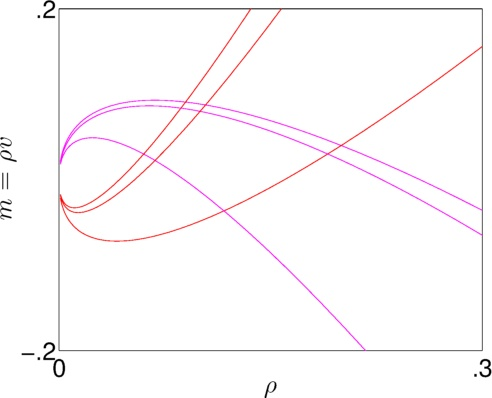
\includegraphics[width=45mm]{../MatlabCode/Images/PW_Loci.jpg}
   }
 \subfigure[Integral curves for $\lambda_1$, $\lambda_2$ shown in light and dark green, respectively.]{
  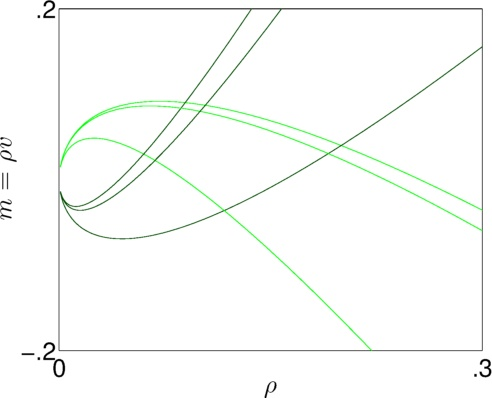
\includegraphics[width=45mm]{../MatlabCode/Images/PW_IntegralCurves.jpg}
   }
 \subfigure[$\lambda_1$ loci and integral curve passing through
  a point $(\rho_*, v_*)$, with $\lambda_1$ contour lines shown in cyan.]{
  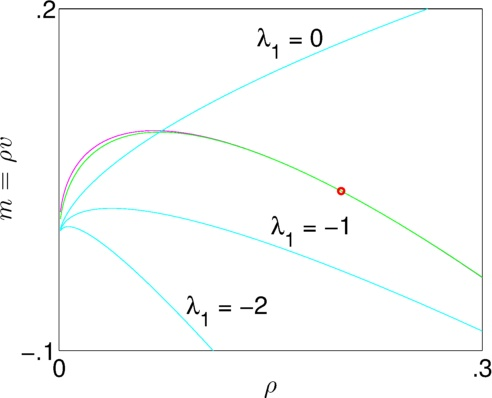
\includegraphics[width=45mm]{../MatlabCode/Images/PW_Lambda1Curves.jpg}
   }
    \subfigure[$\lambda_2$ loci and integral curve passing through
  a point $(\rho_*, v_*)$, with $\lambda_2$ contour lines shown in cyan.]{
  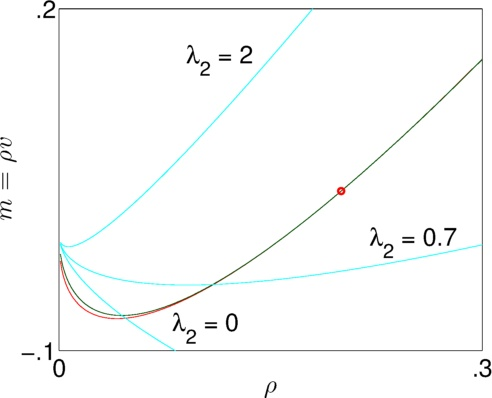
\includegraphics[width=45mm]{../MatlabCode/Images/PW_Lambda2Curves.jpg}
   }
 \subfigure[Valid curves for a point $q_l$.]{
  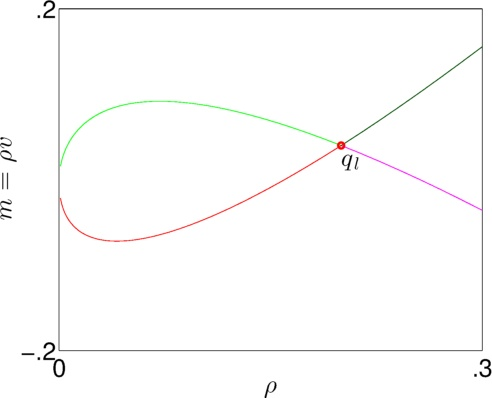
\includegraphics[width=45mm]{../MatlabCode/Images/PW_validStateCurvesLeft.jpg}
   }
 \subfigure[Valid curves for a point $q_r$.]{
  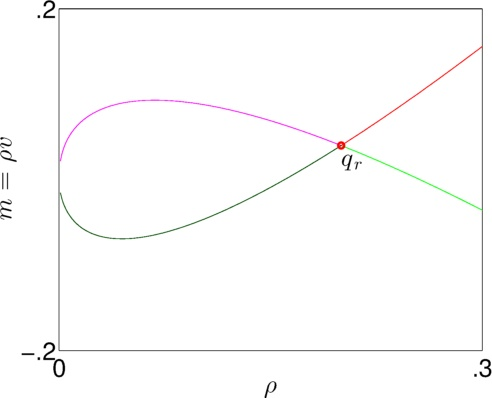
\includegraphics[width=45mm]{../MatlabCode/Images/PW_validStateCurvesRight.jpg}
   }
 \caption[Optional caption for list of figures]
 {Figures of the Hugonio loci and integral curves for $\lambda_1$ and $\lambda_2$ in the $M = (\rho, \rho v)$ plane. Note that loci are shown in red and magenta and integral curves are shown in green.}
  \label{fig:PW_curves}
\end{figure}

Restrictions on the way that $\lambda$ must vary across a wave allow us to identify the regions of the Hugoniot loci and integral curves that are valid for any given point. When traveling across a shock from a left state, $q_l$, to a right state $q_r$, $\lambda$ must decrease. When traveling across a rarefaction wave from a left state, $q_l$, to a right state $q_r$, $\lambda$ must increase. In Figure \ref{fig:PW_curves} (c) and (d) we see the Hugoniot loci and integral curves for this system with the contour lines for $\lambda_1$ and $\lambda_2$. Using these plots, we can determine which areas of the curves are valid shocks and which are valid rarefaction waves. Figure \ref{fig:PW_curves} (e) and (d) shows the points $q_l$ and $q_r$, respectively, with only the valid waves displayed. Here, shocks are shown in red or magenta and rarefaction waves are shown in either light or dark green.

% AR Model
\section{AR Model}

% AR Model: Theory
\subsection{Theory}
To illustrate the PW model's problematic representation of cars as a fluid, Aw and Rascle \cite{AwRascle2000} consider the following situation.  Assume you are in your car, traveling with velocity $v$.  If the density ahead of you is increasing with respect to $x$ but decreasing with respect to $x - vt$, would you speed up or slow down?  Although the cars ahead are more densely spaced, they are traveling faster than you, so you would most likely accelerate.  However, since the density ahead is increasing with respect to $x$, the PW model predicts that you would slow down.  

According to Aw and Rascle, the model should be more concerned with the perspective of the driver, which is relative to a moving frame of reference.  In this case, we should involve the convective derivative of the anticipation factor, $\partial_t + v \partial_x$, instead of the space derivative.  They propose the model:

\[ \left\{ \begin{matrix*}[l] & \rho_t + (\rho v)_x = 0 \\[1ex] & \Big(v + p(\rho)\Big)_t + v \Big(v + p(\rho)\Big)_x = 0 \end{matrix*} \right. \]

In conservative form, the second equation becomes $\Big( \rho (v + p(\rho)) \Big)_t + \Big( \rho v (v + p(\rho)) \Big)_x = 0$.  Aw and Rascle call this conserved quantity, $y = \rho v + \rho p(\rho)$, "momentum", although they admit that $y$ has no obvious physical interpretation. Furthermore, the second equation can also be rewritten as an equation for velocity: $v_t + \Big(v - \rho p'(\rho)\Big)v_x = 0$. If we consider the linearized system,

\[ \begin{pmatrix} \rho \\[1ex] v \end{pmatrix}_t + \begin{pmatrix} v & \rho \\[1ex] 0 & v - \rho p'(\rho) \end{pmatrix} \begin{pmatrix} \rho \\[1ex] v \end{pmatrix}_x = \begin{pmatrix} 0 \\[1ex] 0 \end{pmatrix}, \]

we see that one issues is resolved.  In this model, the largest eigenvalue $\lambda_2 = v$.  Therefore no characteristic speed is greater than the velocity, so that drivers are no longer influenced by conditions behind them. To validate their model, Aw and Rascle claim that their improved model satisfies the following important conditions:
\begin{enumerate}
\item The system is hyperbolic.
\item When solving the Riemann problem with bounded nonnegative data $(\rho, v)$, the density and velocity remain nonnegative and bounded from above.
\item When solving the Riemann problem, no waves connecting any state to its left (behind it) have a propagation speed greater than the velocity $v$.
\item The solution to the Riemann problem agrees with qualitative properties that drivers actually experience: braking produces shock waves and acceleration produces rarefaction waves.
\end{enumerate}

% AR Model: Hugoniot Loci and Integral Curves
\subsection{Hugoniot Loci and Integral Curves}
The AR model starts from the system
\begin{align}
&\partial_t\rho + \partial_x(\rho v) = 0, \label{AR:eq1}\\
&\partial_t \left(v + p(\rho )\right) + v\partial_x \left( v + p(\rho )\right) = 0\label{AR:eq1.5}
\end{align}
with $p(\rho) = \rho^\gamma$.

To find the Hugoniot loci and the integral curves, \cite{AwRascle2000} utilizes two different forms of this system. 
We will examine each of them in turn. What we will find is that the integral curves and the Hugoniot loci coincide, 
and furthermore that one of the waves is a contact discontinuity. Let us first consider the Hugoniot loci. 

\subsubsection{Hugoniot Loci}
In order to consider the Hugoniot loci for this system we must first write the system in conservation form. 
To accomplish this, note that multiplying the first equation by $(v + p(\rho ))$ and the second equation 
by $\rho$ gives us the two equations 
\begin{align*}
&(v + p(\rho ))\partial_t\rho + (v + p(\rho ))\partial_x(\rho v) = 0,  \\
&\rho\partial_t \left(v + p(\rho )\right) + \rho v\partial_x \left( v + p(\rho )\right) = 0.
\end{align*}
Adding these two equations gives
\begin{align}\label{AR:eq2}
\partial_t \left(\rho\left(v + p(\rho )\right)\right) + \partial_x \left( \rho v\left(v + p(\rho )\right)\right) = 0.
\end{align}
Then from (\ref{AR:eq1}) and (\ref{AR:eq2}) we have the system 
\begin{align*}
&\partial_t\rho + \partial_x(\rho v) = 0, \\
&\partial_t \left(\rho\left(v + p(\rho )\right)\right) + \partial_x \left( \rho v\left(v + p(\rho )\right)\right) = 0.
\end{align*}
This can be rewritten as $q_t + f(q)_x = $ by defining
\begin{align*}
q = \left[ \begin{matrix}
\rho \\ y
\end{matrix}\right], \hspace{0.3in}
f(q) = \left[ \begin{matrix}
v\rho \\
vy
\end{matrix}\right].
\end{align*}
where $y = \rho\left(v + p(\rho )\right)$.
The Rankine-Hugoniot condition tells us that 
\begin{align*}
s(q_*- q) = f(q_*) - f(q).
\end{align*}
Therefore, from this condition we get the two equations
\begin{align}
s(\rho_* - \rho) = v_*\rho_* - v\rho, \label{AR:eq3}\\
s(y_* - y) = v_*y_* - vy.\label{AR:eq4}
\end{align}
With a little rearranging and by plugging in for $y$, these two equations can be rewritten as
\begin{align}
&\rho_*(s - v_*) = \rho (s - v), \label{AR:eq5}\\
&\rho_*(s - v_*)\left(v_* + p(\rho_* )\right) = \rho(s - v)\left(v + p(\rho )\right).\label{AR:eq6}
\end{align}
From (\ref{AR:eq5}), we know that there are two cases: 

(a) $\rho_*(s - v_*) = \rho (s - v) = 0$. In this case we have that
\begin{align*}
s - v_* = s - v 
\end{align*}
except if one of the two densities, $\rho_*$, $\rho$ is zero. Therefore, we can say that
\begin{align*}
v_* = v.
\end{align*}
Since the velocity does not change, this is a contact discontinuity. Using the fact that $v = v_*$ in (\ref{AR:eq4}) gives
\begin{align*}
y_*(s - v) = y(s - v).
\end{align*}
So, either $y = y_*$ or $s = v$. If $y = y_*$ we have a stationary point in the $Y = (\rho, y)$ plane, which does not 
describe a wave. Therefore, $s = v$. Note that we have no restrictions on $y$ other than its definition. 
Therefore this loci in the $Y$ plane is given by 
\begin{align*}
y = \rho ( v_* + p(\rho )).
\end{align*}

\begin{figure}[H]
 \centering
    \subfigure[$\lambda_1$-curves.]{
  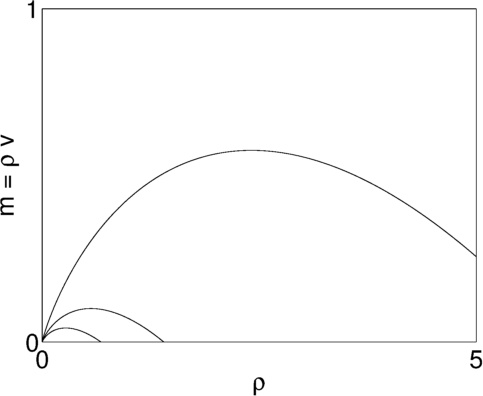
\includegraphics[width=45mm]{../MatlabCode/Images/HLIC_M_lamb1.jpg}
   }
 \subfigure[$\lambda_2$-curves.]{
  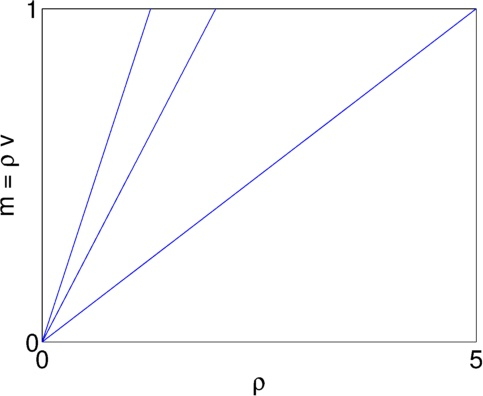
\includegraphics[width=45mm]{../MatlabCode/Images/HLIC_M_lamb2.jpg}
   }
 \subfigure[$\lambda_1$-curve and $\lambda_2$-curve passing through 
 the point $(\rho_*,m_*)$.]{
  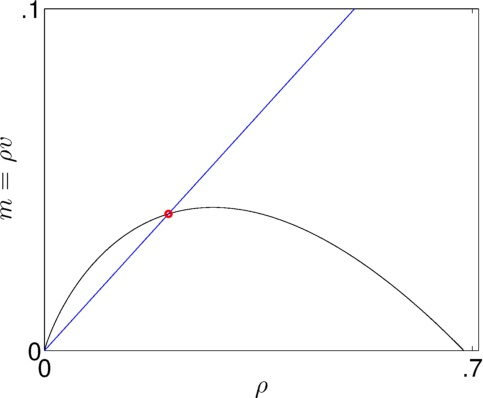
\includegraphics[width=45mm]{../MatlabCode/Images/HLIC_M.jpg}
   }
 \caption[Optional caption for list of figures]
 {Figures of the Hugonio loci and integral curves for $\lambda_1$ and $\lambda_2$. 
 Since the loci and integral curves coincide, they are 
 both simply called the ``curves'' in the captions of the above figures. 
 Figure (c) shows both curves for a given point.}
  \label{fig:AR_curves}
\end{figure}

(b) $\rho_*(s - v_*) = \rho (s - v) \neq 0$. In this case, plugging this into (\ref{AR:eq6}) gives
\begin{align*}
\rho_*(s - v_*)\left(v_* + p(\rho_* )\right) &= \rho(s - v)\left(v + p(\rho )\right)\\
\rho(s - v)\left(v_* + p(\rho_* )\right) &= \rho(s - v)\left(v + p(\rho )\right)\\
v_* + p(\rho_* )&= v + p(\rho ).
\end{align*}
Therefore, the Hugoniot loci for this case in the Y plane are given by
\begin{align*}
y = v_* + p(\rho_* ),
\end{align*}
since $y = v + p(\rho )$ by definition. Note that solving (\ref{AR:eq3}) for $s$ gives
\begin{align*}
s = \frac{\rho_*v_* - \rho v}{\rho_* - \rho}.
\end{align*}
Using the fact that $v_* = v + p(\rho) - p(\rho_*)$, we get that
\begin{align*}
s = \frac{\rho_*\left( v + p(\rho) - p(\rho_*)\right)- \rho v}{\rho_* - \rho}
= v - \rho_*\frac{p(\rho ) - p(\rho_*)}{\rho - \rho_*}
\approx v - \rho p'(\rho)
\end{align*}
for $\rho_* \approx \rho$. 

In the $U = (\rho, v)$ plane these loci become (a) $v = v_*$, $\rho$ free, and (b) $v = v_* + p(\rho_* ) - p(\rho )$.
 In the $M = (\rho, \rho v)$ plane these loci become (a) $\rho v = \rho_* v_*$, $\rho$ free, 
 and (b) $\rho v = \rho \left( v_* + p(\rho_*)\right) - \rho p(\rho))$. Figure \ref{fig:AR_curves} shows the Hugoniot loci 
 in the different planes. TODO: ADD PARAMETERS USED FOR FIGURES? OR, WILL INCLUDING THE CODE MAKE THAT REDUNDANT? 
 IF WE ADD PARAMETERS, MAYBE THE BEST PRESENTATION WOULD BE IN A TABLE?

\subsubsection{Integral Curves}
In order to consider the integral curves for this system \cite{AwRascle2000} 
works from the system
\begin{align*}
&\partial_t \rho + \partial_x (\rho v) = 0 \\ 
&\partial_t v + \left(v - p'(\rho)\rho\right)\partial_x v = 0,
\end{align*}
where the second equation is found by multiplying (\ref{AR:eq1}) 
by $p'(\rho)$ and subtracting it from (\ref{AR:eq1.5}). 
This can be rewritten as $q_t + Aq_t = 0$ by defining
\begin{align*}
q = \left[ \begin{matrix}
\rho \\ v
\end{matrix}\right] , \hspace{0.3in}
A = \left[ \begin{matrix}
v & \rho \\
0 & v - p'(\rho ) \rho
\end{matrix}\right].
\end{align*}
The eigenvalues of $A$ are $\lambda_1 = v - p'(\rho ) \rho$ and 
$\lambda_2 = v$. Note that since $p(\rho ) = \rho^{\gamma}$ 
and $\rho \geq 0$, $\lambda_1 < \lambda_2$ so long as $\rho \neq 0$. 
Also note that if $\rho = 0$ then $A$ is no longer 
hyperbolic. The eigenvectors of $A$ are
\begin{align*}
r_1 = \left[ \begin{matrix}
1 \\ - p'(\rho )
\end{matrix}\right], \hspace{0.3in}
r_2 = \left[ \begin{matrix}
1 \\ 0
\end{matrix}\right].
\end{align*}
Using equation (13.24) from \cite{LeVeque2002} with $\alpha = 1$ tells us 
that the integral curves can be found by considering $q'(\xi ) = r_p$. 
For $p = 1$ this gives us the two equations
\begin{align*}
&\rho'(\xi ) = 1 \\
&v'(\xi ) = - p'(\rho ),
\end{align*}
which can be solved to find that we have parameratized our curve by $\rho$, 
and $v = - p'(\rho ) + c_1$ while $\rho$ is free, where $c_1$ is a constant. 
Since for a given point $(\rho_*, v_*)$ when $\rho = \rho_*$ we want 
$v = v_*$, we get that $c_1 = v_* + p'(\rho_*)$. Thus, the integral curve 
is given by 
\begin{align*}
v = v_* + p'(\rho_*) - p'(\rho ).
\end{align*}
This coincides with the Hugoniot loci from case (b). For $p = 2$, we get the 
two equations
\begin{align*}
&\rho'(\xi ) = 1 \\
&v'(\xi ) = 0,
\end{align*}
which can be solved to find that we have parameratized our curve by $\rho$, 
and that $v$ is a constant. Therefore, $v = v_*$ and $\rho$ is free. 
This coincides with the Hugoniot loci from case (a).

\begin{figure}[H]
 \centering
    \subfigure[$\lambda_1$-curves with contours of $\lambda_1$.]{
  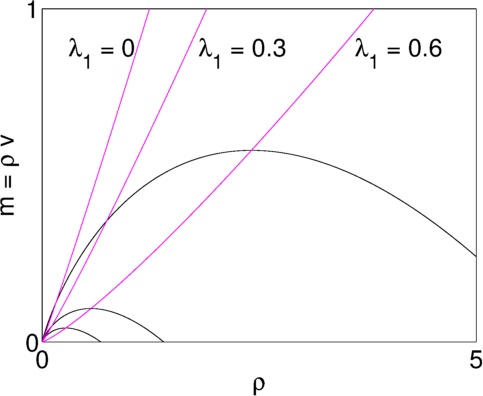
\includegraphics[width=45mm]{../MatlabCode/Images/Validity_M.jpg}
   }
 \subfigure[Valid waves for the point $q_l$.]{
  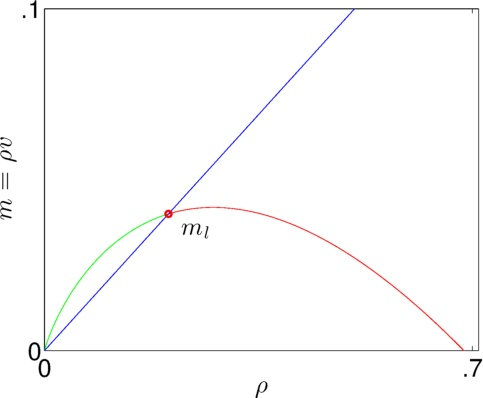
\includegraphics[width=45mm]{../MatlabCode/Images/Validity_M_ql.jpg}
   }
 \subfigure[Valid waves for the point $q_r$.]{
  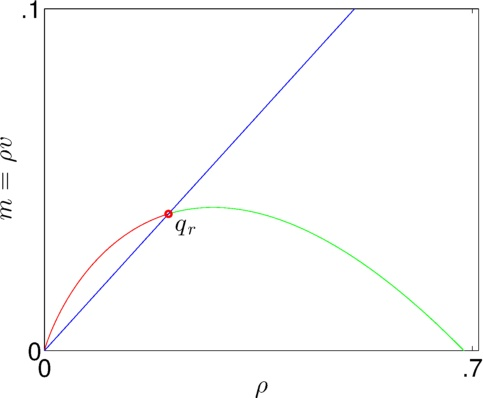
\includegraphics[width=45mm]{../MatlabCode/Images/Validity_M_qr.jpg}
   }
 \caption[Optional caption for list of figures]
 {Figures showing the calculation of the valid waves for a given point. Figures (a)
  and (d) show the $\lambda_1$ curves in black with the $\lambda_1$ contours 
  in cyan. The other figures show valid shocks in red and valid rarefaction 
  waves in green. The contact discontinuity is shown in blue.}
   \label{fig:AR_validity}
\end{figure}

\subsubsection{Regions of Validity}
Restrictions on the way that $\lambda$ must vary across a wave allow us to identify the regions of the Hugoniot loci and integral curves that are valid for any given point. When traveling across a shock from a left state, $q_l$, to a right state $q_r$, $\lambda$ must decrease. When traveling across a rarefaction wave from a left state, $q_l$, to a right state $q_r$, $\lambda$ must increase. 

Therefore, it is important to take into account the contour lines of $\lambda$ when 
looking at the loci and integral curves. Figures \ref{fig:AR_validity}(a) and 
\ref{fig:AR_validity}(d) show the $\lambda_1$-curves in the $U$ and $M$ planes,
with the contour lines of $\lambda_1$ shown in magenta. This information is used
to determine which areas of the $\lambda_1$ curves are valid shock waves and which
are valid rarefaction waves. The rest of the subfigures show the regions of validity for 
specific points $q_*$, depending on whether $q_* = q_l$ or $q_* = q_r$. For these plots,
$q_* = (\rho_*,v_*) = (0.2, 0.2)$. Note that the contact discontinuity is valid
anywhere in the plane. 

% Examples
\section{Examples}

\begin{figure}[H]
 \centering
 \subfigure[Solution from the AR model.]{
  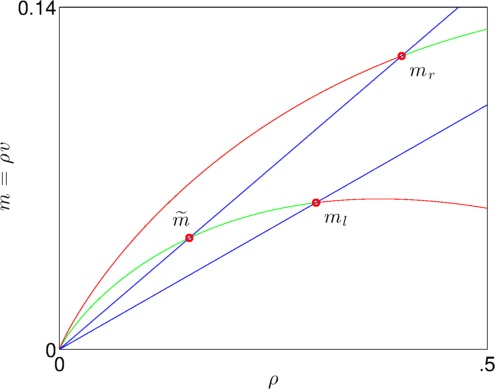
\includegraphics[width=70mm]{../MatlabCode/Images/AR_example1.jpg}
   }
    \subfigure[Solution from the PW model.]{
  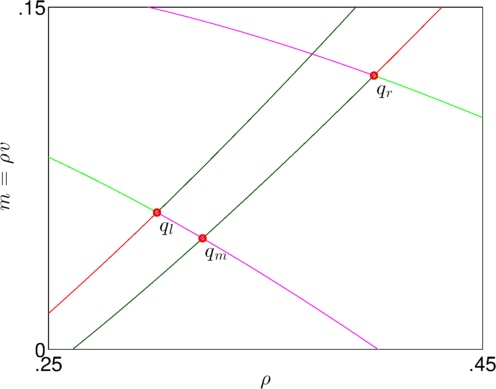
\includegraphics[width=70mm]{../MatlabCode/Images/PW_example1.jpg}
   }
 \caption[Optional caption for list of figures]
 {Solutions to the Riemann problem for example 1 from the AR and PW models.}
  \label{fig:example1}
\end{figure}

\begin{figure}[H]
 \centering
 \subfigure[Solution from the AR model.]{
  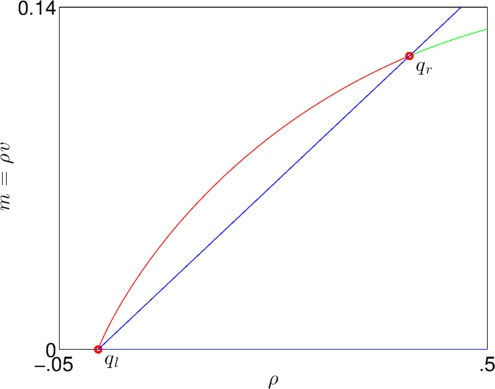
\includegraphics[width=70mm]{../MatlabCode/Images/AR_example2.jpg}
   }
 \subfigure[Solution from the PW model.]{
  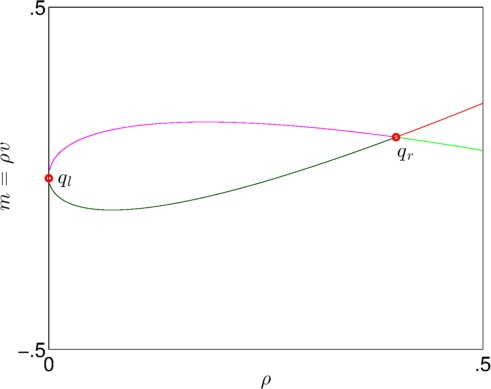
\includegraphics[width=70mm]{../MatlabCode/Images/PW_example2.jpg}
   }
 \caption[Optional caption for list of figures]
 {Solutions to the Riemann problem for example 2 from the AR and PW models.}
  \label{fig:example2}
\end{figure}

\begin{table}[t]
\caption{Initial values used in examples 1 and 2.}
\begin{center}
\begin{tabular}{| c | c c  c c|}
\hline
& $v_l$ & $\rho_l $ & $v_r$ & $\rho_r $\\
\hline
Example 1 & 0.2 & .03 & 0.3 & 0.4 \\
Example 2 & 0 & 0 & 0.3 & 0.4\\
\hline
\end{tabular}
\end{center}
 \label{table:1}
\end{table}

Reproducing the Riemann problems found in \cite{AwRascle2000}, we consider two different examples. The variables used in these two examples are shown in Table \ref{table:1}. Note that in the solution from the AR model for example 1, shown in Figure \ref{fig:example1} (a), the transition from $q_l = (\rho_l, v_l\rho_l)$ to $q_r = (\rho_r, v_r\rho_r)$ is first a shock and then a contact discontinuity. The middle state is denoted by $q_m$ in the figure. In the solution given by the AR model for example 2, show in Figure \ref{fig:example2} (a), the transition from $q_l = (\rho_l, v_l\rho_l)$ to $q_r = (\rho_r, v_r\rho_r)$ is a shock wave, and there is no middle state.

In both examples the density and velocity are greater in the right state than in the left state.  This corresponds to the situation considered by Aw and Rascle that motivated the use of the convective derivative.  In the first example, we see that the AR model predicts that the density of the middle state is less than both left or right states, but that the velocity increases steadily from left state to right.  This is what we would expect, as drivers spread out as the accelerate to catch up with the cars ahead.  On the other hand, the PW model predicts that the middle state will have a greater density than the left state but a smaller velocity.  This is opposite of what we would expect.

In the second example, we consider the case where there are no cars on the left.  Once again the AR model predicts what we would expect.  Here the cars continue to move to the right at a constant velocity, while the state on the left remains zero.  Note that in Clawpack solutions the density and velocity are undefined in the middle, but that this is a result of numerical issues.  In reality they should both be zero.  The PW method again fails to produce reasonable results.  Not only does it predict negative velocities, but we can see from the density plot that some cars have in fact moved backwards into the left region.  While it would make sense for fluids to act this way, we do not expect drivers to start moving in reverse when they see that nobody is behind them!

\begin{figure}[H]
 \centering
 \subfigure[Solution from the AR model.]{
  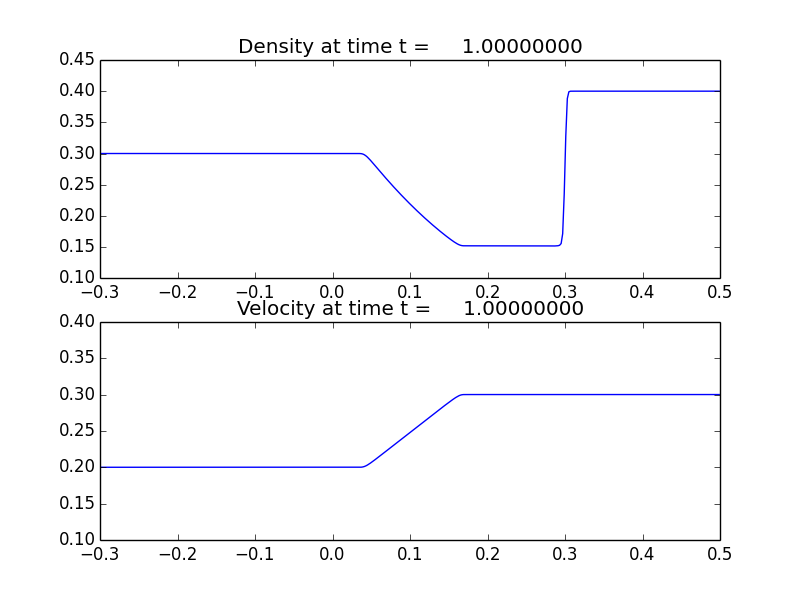
\includegraphics[width=70mm]{../ClawpackCode/AR/ARexample1.png}
   }
 \subfigure[Solution from the PW model.]{
  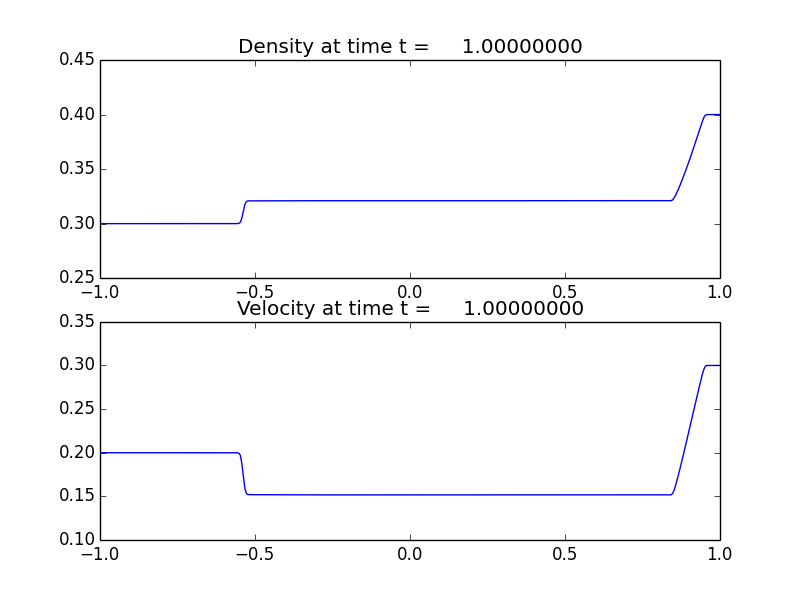
\includegraphics[width=70mm]{../ClawpackCode/PW/PWexample1.png}
   }
 \caption[Optional caption for list of figures]
 {Solutions to the Riemann problem for example 1 computed in Clawpack.}
  \label{fig:example2}
\end{figure}

\begin{figure}[H]
 \centering
 \subfigure[Solution from the AR model.]{
  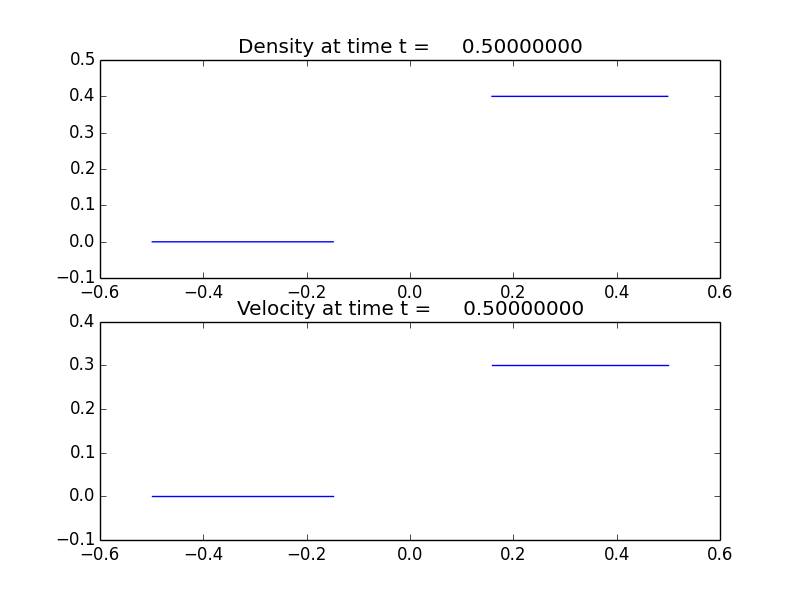
\includegraphics[width=70mm]{../ClawpackCode/AR/ARexample2.png}
   }
 \subfigure[Solution from the PW model.]{
  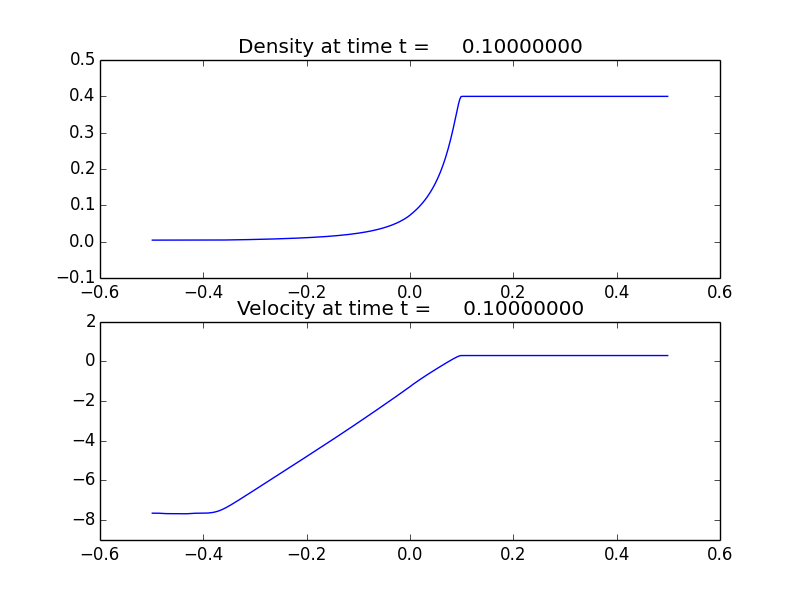
\includegraphics[width=70mm]{../ClawpackCode/PW/PWexample2.png}
   }
 \caption[Optional caption for list of figures]
 {Solutions to the Riemann problem for example 2 computed in Clawpack.}
  \label{fig:example2}
\end{figure}

\section{Conclusion}
By studying the examples of the LWR, PW and AR models for traffic flow, we see that higher order models are not always more accurate than first order models.  Additionally, the assumptions made in developing higher order relations must conform to the phenomena they are designed to model.  For example, using equations for isotropic fluids to model anisotropic cars in the PW model produces nonphysical results.  The AR model corrects this problem by using a convective derivative rather than a space derivative for the anticipation factor.  Therefore, whenever we introduce higher order models, we should follow the example of Aw and Rascle by validating the model's results in a systematic way.  

\bibliography{Draft}{}
\bibliographystyle{plain}
\end{document}